\documentclass{../uafthesis}

\usepackage{amsmath, amssymb, amsfonts} % Thanks, AMS!
\usepackage{fixltx2e} % Allows \(\) in captions, amongst other things.
%\usepackage{ppl} % The Paladino font (tough to find?)
\usepackage{pxfonts} % Paladino-like fonts
\usepackage{graphicx, float} % Graphics stuff
\usepackage{verbatim} % Mostly for the comment environment.
%\usepackage{chapterbib} % This is an option for those bundling papers.
\usepackage[square]{natbib}
%\usepackage{tocbibind} % This fixes the "bibliography in ToC" problem.
                        % Use with chapterbib.
\usepackage{url} % I quote some URLs in the bibliography"

\renewcommand{\cite}[1]{\citep{#1}}


\begin{document}

\title{An Example Thesis Document}
\author{Joshua Holbrook}

\degreeyear{2011}
\degreemonth{May}
\degree{Master of Arts}
\department{Dept. of Fresh Beats}
\numberofmembers{3} % Make sure this is right! The grad school hates empty
                    % signature lines.
\committeewidth{4in}
\approvedwidth{4in}
\comitteespace{\hfill}
\approvedspace{\hfill}

\prevdegrees{B.A.M.F.}
\college{College of Pwning Noobs}


\makesig
\maketitle

% Wondering when to use `input' and when to use `include?'
% read http://en.wikibooks.org/wiki/LaTeX/Basics#Big_Projects .
\begin{abstract}
  \input abstract.tex
\end{abstract}


%Table of Contents and such
\tableofcontents
\listoffigures
\listoftables
%\listofothermaterials
\listofappendices

\begin{acknowledgements}
  \input acknowledgements.tex
\end{acknowledgements}

\begin{quotepage}
  \input quotepage.tex
\end{quotepage}

\chapter{What's All This, Then?}

\section{Introduction}

This is the project for the \texttt{uafthesis} \LaTeX document class, the
official unofficial volunteer-driven document class for theses written for the
University of Alaska Fairbanks, in \LaTeX.

\section{Prerequisites}

Before you decide to write your thesis in \LaTeX, you should already know a
little \LaTeX and feel comfortable writing and compiling a simple document,
especially one with figures and tables.

Additionally, you will have to use \texttt{bibtex} (or some alternative) to keep
track of references. It's not particularly difficult, but chances are you will
have to either learn it or give yourself a refresher.

One thing you will see in this example that you may not have encountered before
is the use of \textbackslash input and \textbackslash include to split the project into multiple, smaller
files. The most important difference is that \textbackslash include will wrap the included
file in page-breaks, while \textbackslash input may as well be a copy-paste job.

Another issue that may come up is having to run \texttt{pdflatex} and
\texttt{bibtex} multiple times. In order to do a full compile without anything
wrong, you will have to run something like the following commands:

\begin{verbatim}
pdflatex example
pdflatex example
pdflatex example
bibtex example
pdflatex example
pdflatex example
\end{verbatim}

That's right, \texttt{pdflatex} gets ran five times. A similar situation arises
from the use of vanilla \texttt{latex}. This is because of how \LaTeX generates
files while compiling that it uses to fill in data during subsequent 
run-throughs.

This can be mitigated somewhat by using some sort of build system. For example,
Ryan Woodard advocated using a makefile to ease the pain. Another option may
be Rubber, or even the full set of commands in a shell script. There are many
techniques, some more appropriate than others. \cite{buildsystems}

It is also worth your time to read other theses, to get an idea of how they
should be written. This may seem obvious, but I will admit that I did not, and
I ended up going through many a rewrite. Also obvious: This document is
\emph{not} written like a thesis. Duh.

Finally, \textbf{at least skim the UAF Thesis Handbook}. \cite{handbook} It's
not hard, and it will give you an idea of what to expect in terms of formatting.
In particular, as \texttt{uafthesis} is a volunteer effort, \emph{there is no
guarantee that the graduate school's formatting guidelines are met by this
document class.} Moreover, some things (such as proper initial capitals in title
headings) are on you, and not something \texttt{uafthesis} does for you.


\section{Installation}

Like any \LaTeX files, there are basically two ways:

\begin{itemize}
\item Copy \texttt{uafthesis.cls} into the same folder as your project. This is
probably the easiest way.
\item Set yourself up with a properly indexed \texttt{~/texmf/latex} folder,
create a new folder called ``uafthesis,'' and put \texttt{uafthesis.cls} into
that folder. This involves some initial effort, but if you use \LaTeX regularly
it's worthwhile for holding all sorts of packages. In fact, if you are a
regular \LaTeX user, you may have already done this.
\end{itemize}

Which method you choose is up to you.

\chapter{Basic Use}

\section{Introduction}

In this section, I take the main file, show some snippets, and explain what
they all mean, or why you would want to use these things.

\section{example.tex}

\begin{verbatim}
\documentclass{uafthesis}
\end{verbatim}

This is where the secret sauce is.

\begin{verbatim}
\usepackage{fixltx2e} % Allows \(\) in captions, amongst other things.
\usepackage{ppl} % The Paladino font
\usepackage{amsmath, amssymb, amsfonts} % Thanks, AMS!
\usepackage{graphicx, float} % Graphics stuff
\usepackage{verbatim} % For very basic listings and multi-line comments.
%\usepackage{chapterbib} % This is an option for those bundling papers.
\usepackage[square]{natbib}
%\usepackage{tocbibind} % This fixes the "bibliography in ToC" problem.
                        % Use with chapterbib.
\usepackage{url} % I quote some URLs in the bibliography"
\end{verbatim}

\texttt{fixltx2e} fixes an annoying bug where using inline mathematics
delimiters in captions for graphics and tables would cause errors in the
compiler. Alternately, one may simply use the dollar signs instead.

\texttt{ppl} is the ``Paladino'' font, which has been extremely popular for
UAF theses in the past. There is, however, no rule against using ``Computer
Modern'' or some other font, and in fact ``Paladino'' was originally intended
for headings only when it was designed (fun fact).

Some writers of theses end up bundling multiple published papers into a thesis,
especially in the case of PhD candidates. \texttt{chapterbib} allows for
separate bibliographies for each chapter, which is the most appropriate format
given this bundled-paper style of thesis. Many theses---mine included---only
have a single bibliography.

Finally, \texttt{natbib} allows one to change how citations appear.

\small
\begin{verbatim}
\renewcommand{\cite}[1]{\citep{#1}}

\end{verbatim}
\normalsize

Many authors write their own \LaTeX macros in order to make writing their thesis
easier. This document does not have any custom macros.

\small
\begin{verbatim}
\begin{document}

\title{An Example Thesis Document}
\author{Joshua Holbrook}

\degreeyear{2011}
\degreemonth{May}
\degree{Master of Arts}
\department{Dept. of Fresh Beats}
\numberofmembers{3} % Make sure this is right! The grad school hates empty
                    % signature lines.
\prevdegrees{B.A.M.F.}
\college{College of Pwning Noobs}

\makesig
\maketitle
\end{verbatim}
\normalsize

In this section, the important information about the thesis is filled in, and
then the signature page and title page are generated.

\small
\begin{verbatim}
% Wondering when to use `input' and when to use `include?'
% read http://en.wikibooks.org/wiki/LaTeX/Basics#Big_Projects .
\begin{abstract}
  \input abstract.tex
\end{abstract}

%Table of Contents and such
\tableofcontents
\listoffigures
\listoftables
%\listofothermaterials
\listofappendices
\end{verbatim}
\normalsize

Here, the abstract is inserted, then the table of contents and other tables.
Note that the appendices are in a separate table. \textbf{This is not typical}
in \LaTeX and requires special handling, as detailed in the next chapter.
Similarly with the List of Other Materials, if your thesis has one (think
CDs and such).

\small
\begin{verbatim}
\begin{acknowledgements}
  \input acknowledgements.tex
\end{acknowledgements}

\begin{quotepage}
  \input quotepage.tex
\end{quotepage}

\chapter{What's All This, Then?}

\section{Introduction}

This is the project for the \texttt{uafthesis} \LaTeX document class, the
official unofficial volunteer-driven document class for theses written for the
University of Alaska Fairbanks, in \LaTeX.

\section{Prerequisites}

Before you decide to write your thesis in \LaTeX, you should already know a
little \LaTeX and feel comfortable writing and compiling a simple document,
especially one with figures and tables.

Additionally, you will have to use \texttt{bibtex} (or some alternative) to keep
track of references. It's not particularly difficult, but chances are you will
have to either learn it or give yourself a refresher.

One thing you will see in this example that you may not have encountered before
is the use of \textbackslash input and \textbackslash include to split the project into multiple, smaller
files. The most important difference is that \textbackslash include will wrap the included
file in page-breaks, while \textbackslash input may as well be a copy-paste job.

Another issue that may come up is having to run \texttt{pdflatex} and
\texttt{bibtex} multiple times. In order to do a full compile without anything
wrong, you will have to run something like the following commands:

\begin{verbatim}
pdflatex example
pdflatex example
pdflatex example
bibtex example
pdflatex example
pdflatex example
\end{verbatim}

That's right, \texttt{pdflatex} gets ran five times. A similar situation arises
from the use of vanilla \texttt{latex}. This is because of how \LaTeX generates
files while compiling that it uses to fill in data during subsequent 
run-throughs.

This can be mitigated somewhat by using some sort of build system. For example,
Ryan Woodard advocated using a makefile to ease the pain. Another option may
be Rubber, or even the full set of commands in a shell script. There are many
techniques, some more appropriate than others. \cite{buildsystems}

It is also worth your time to read other theses, to get an idea of how they
should be written. This may seem obvious, but I will admit that I did not, and
I ended up going through many a rewrite. Also obvious: This document is
\emph{not} written like a thesis. Duh.

Finally, \textbf{at least skim the UAF Thesis Handbook}. \cite{handbook} It's
not hard, and it will give you an idea of what to expect in terms of formatting.
In particular, as \texttt{uafthesis} is a volunteer effort, \emph{there is no
guarantee that the graduate school's formatting guidelines are met by this
document class.} Moreover, some things (such as proper initial capitals in title
headings) are on you, and not something \texttt{uafthesis} does for you.


\section{Installation}

Like any \LaTeX files, there are basically two ways:

\begin{itemize}
\item Copy \texttt{uafthesis.cls} into the same folder as your project. This is
probably the easiest way.
\item Set yourself up with a properly indexed \texttt{~/texmf/latex} folder,
create a new folder called ``uafthesis,'' and put \texttt{uafthesis.cls} into
that folder. This involves some initial effort, but if you use \LaTeX regularly
it's worthwhile for holding all sorts of packages. In fact, if you are a
regular \LaTeX user, you may have already done this.
\end{itemize}

Which method you choose is up to you.

\chapter{Basic Use}

\section{Introduction}

In this section, I take the main file, show some snippets, and explain what
they all mean, or why you would want to use these things.

\section{example.tex}

\begin{verbatim}
\documentclass{uafthesis}
\end{verbatim}

This is where the secret sauce is.

\begin{verbatim}
\usepackage{fixltx2e} % Allows \(\) in captions, amongst other things.
\usepackage{ppl} % The Paladino font
\usepackage{amsmath, amssymb, amsfonts} % Thanks, AMS!
\usepackage{graphicx, float} % Graphics stuff
\usepackage{verbatim} % For very basic listings and multi-line comments.
%\usepackage{chapterbib} % This is an option for those bundling papers.
\usepackage[square]{natbib}
%\usepackage{tocbibind} % This fixes the "bibliography in ToC" problem.
                        % Use with chapterbib.
\usepackage{url} % I quote some URLs in the bibliography"
\end{verbatim}

\texttt{fixltx2e} fixes an annoying bug where using inline mathematics
delimiters in captions for graphics and tables would cause errors in the
compiler. Alternately, one may simply use the dollar signs instead.

\texttt{ppl} is the ``Paladino'' font, which has been extremely popular for
UAF theses in the past. There is, however, no rule against using ``Computer
Modern'' or some other font, and in fact ``Paladino'' was originally intended
for headings only when it was designed (fun fact).

Some writers of theses end up bundling multiple published papers into a thesis,
especially in the case of PhD candidates. \texttt{chapterbib} allows for
separate bibliographies for each chapter, which is the most appropriate format
given this bundled-paper style of thesis. Many theses---mine included---only
have a single bibliography.

Finally, \texttt{natbib} allows one to change how citations appear.

\small
\begin{verbatim}
\renewcommand{\cite}[1]{\citep{#1}}

\end{verbatim}
\normalsize

Many authors write their own \LaTeX macros in order to make writing their thesis
easier. This document does not have any custom macros.

\small
\begin{verbatim}
\begin{document}

\title{An Example Thesis Document}
\author{Joshua Holbrook}

\degreeyear{2011}
\degreemonth{May}
\degree{Master of Arts}
\department{Dept. of Fresh Beats}
\numberofmembers{3} % Make sure this is right! The grad school hates empty
                    % signature lines.
\prevdegrees{B.A.M.F.}
\college{College of Pwning Noobs}

\makesig
\maketitle
\end{verbatim}
\normalsize

In this section, the important information about the thesis is filled in, and
then the signature page and title page are generated.

\small
\begin{verbatim}
% Wondering when to use `input' and when to use `include?'
% read http://en.wikibooks.org/wiki/LaTeX/Basics#Big_Projects .
\begin{abstract}
  \input abstract.tex
\end{abstract}

%Table of Contents and such
\tableofcontents
\listoffigures
\listoftables
%\listofothermaterials
\listofappendices
\end{verbatim}
\normalsize

Here, the abstract is inserted, then the table of contents and other tables.
Note that the appendices are in a separate table. \textbf{This is not typical}
in \LaTeX and requires special handling, as detailed in the next chapter.
Similarly with the List of Other Materials, if your thesis has one (think
CDs and such).

\small
\begin{verbatim}
\begin{acknowledgements}
  \input acknowledgements.tex
\end{acknowledgements}

\begin{quotepage}
  \input quotepage.tex
\end{quotepage}

\chapter{What's All This, Then?}

\section{Introduction}

This is the project for the \texttt{uafthesis} \LaTeX document class, the
official unofficial volunteer-driven document class for theses written for the
University of Alaska Fairbanks, in \LaTeX.

\section{Prerequisites}

Before you decide to write your thesis in \LaTeX, you should already know a
little \LaTeX and feel comfortable writing and compiling a simple document,
especially one with figures and tables.

Additionally, you will have to use \texttt{bibtex} (or some alternative) to keep
track of references. It's not particularly difficult, but chances are you will
have to either learn it or give yourself a refresher.

One thing you will see in this example that you may not have encountered before
is the use of \textbackslash input and \textbackslash include to split the project into multiple, smaller
files. The most important difference is that \textbackslash include will wrap the included
file in page-breaks, while \textbackslash input may as well be a copy-paste job.

Another issue that may come up is having to run \texttt{pdflatex} and
\texttt{bibtex} multiple times. In order to do a full compile without anything
wrong, you will have to run something like the following commands:

\begin{verbatim}
pdflatex example
pdflatex example
pdflatex example
bibtex example
pdflatex example
pdflatex example
\end{verbatim}

That's right, \texttt{pdflatex} gets ran five times. A similar situation arises
from the use of vanilla \texttt{latex}. This is because of how \LaTeX generates
files while compiling that it uses to fill in data during subsequent 
run-throughs.

This can be mitigated somewhat by using some sort of build system. For example,
Ryan Woodard advocated using a makefile to ease the pain. Another option may
be Rubber, or even the full set of commands in a shell script. There are many
techniques, some more appropriate than others. \cite{buildsystems}

It is also worth your time to read other theses, to get an idea of how they
should be written. This may seem obvious, but I will admit that I did not, and
I ended up going through many a rewrite. Also obvious: This document is
\emph{not} written like a thesis. Duh.

Finally, \textbf{at least skim the UAF Thesis Handbook}. \cite{handbook} It's
not hard, and it will give you an idea of what to expect in terms of formatting.
In particular, as \texttt{uafthesis} is a volunteer effort, \emph{there is no
guarantee that the graduate school's formatting guidelines are met by this
document class.} Moreover, some things (such as proper initial capitals in title
headings) are on you, and not something \texttt{uafthesis} does for you.


\section{Installation}

Like any \LaTeX files, there are basically two ways:

\begin{itemize}
\item Copy \texttt{uafthesis.cls} into the same folder as your project. This is
probably the easiest way.
\item Set yourself up with a properly indexed \texttt{~/texmf/latex} folder,
create a new folder called ``uafthesis,'' and put \texttt{uafthesis.cls} into
that folder. This involves some initial effort, but if you use \LaTeX regularly
it's worthwhile for holding all sorts of packages. In fact, if you are a
regular \LaTeX user, you may have already done this.
\end{itemize}

Which method you choose is up to you.

\chapter{Basic Use}

\section{Introduction}

In this section, I take the main file, show some snippets, and explain what
they all mean, or why you would want to use these things.

\section{example.tex}

\begin{verbatim}
\documentclass{uafthesis}
\end{verbatim}

This is where the secret sauce is.

\begin{verbatim}
\usepackage{fixltx2e} % Allows \(\) in captions, amongst other things.
\usepackage{ppl} % The Paladino font
\usepackage{amsmath, amssymb, amsfonts} % Thanks, AMS!
\usepackage{graphicx, float} % Graphics stuff
\usepackage{verbatim} % For very basic listings and multi-line comments.
%\usepackage{chapterbib} % This is an option for those bundling papers.
\usepackage[square]{natbib}
%\usepackage{tocbibind} % This fixes the "bibliography in ToC" problem.
                        % Use with chapterbib.
\usepackage{url} % I quote some URLs in the bibliography"
\end{verbatim}

\texttt{fixltx2e} fixes an annoying bug where using inline mathematics
delimiters in captions for graphics and tables would cause errors in the
compiler. Alternately, one may simply use the dollar signs instead.

\texttt{ppl} is the ``Paladino'' font, which has been extremely popular for
UAF theses in the past. There is, however, no rule against using ``Computer
Modern'' or some other font, and in fact ``Paladino'' was originally intended
for headings only when it was designed (fun fact).

Some writers of theses end up bundling multiple published papers into a thesis,
especially in the case of PhD candidates. \texttt{chapterbib} allows for
separate bibliographies for each chapter, which is the most appropriate format
given this bundled-paper style of thesis. Many theses---mine included---only
have a single bibliography.

Finally, \texttt{natbib} allows one to change how citations appear.

\small
\begin{verbatim}
\input{custom-macros.tex}
\end{verbatim}
\normalsize

Many authors write their own \LaTeX macros in order to make writing their thesis
easier. This document does not have any custom macros.

\small
\begin{verbatim}
\begin{document}

\title{An Example Thesis Document}
\author{Joshua Holbrook}

\degreeyear{2011}
\degreemonth{May}
\degree{Master of Arts}
\department{Dept. of Fresh Beats}
\numberofmembers{3} % Make sure this is right! The grad school hates empty
                    % signature lines.
\prevdegrees{B.A.M.F.}
\college{College of Pwning Noobs}

\makesig
\maketitle
\end{verbatim}
\normalsize

In this section, the important information about the thesis is filled in, and
then the signature page and title page are generated.

\small
\begin{verbatim}
% Wondering when to use `input' and when to use `include?'
% read http://en.wikibooks.org/wiki/LaTeX/Basics#Big_Projects .
\begin{abstract}
  \input abstract.tex
\end{abstract}

%Table of Contents and such
\tableofcontents
\listoffigures
\listoftables
%\listofothermaterials
\listofappendices
\end{verbatim}
\normalsize

Here, the abstract is inserted, then the table of contents and other tables.
Note that the appendices are in a separate table. \textbf{This is not typical}
in \LaTeX and requires special handling, as detailed in the next chapter.
Similarly with the List of Other Materials, if your thesis has one (think
CDs and such).

\small
\begin{verbatim}
\begin{acknowledgements}
  \input acknowledgements.tex
\end{acknowledgements}

\begin{quotepage}
  \input quotepage.tex
\end{quotepage}

\include{ch1}
\include{ch2}
\include{ch3}
\end{verbatim}
\normalsize

After inputting a few more pages, the chapters (separate documents) are all
included.

\small
\begin{verbatim}
\nocite{wikibook}
\bibliographystyle{agufull08}
\bibliography{thesis}
\end{verbatim}
\normalsize

This generates the bibliography. Note that the bibliography style is set to
\texttt{agufull08}. Generally, the graduate school isn't picky about 
bibliography style, as long as it's consistent. For geophysics papers (very
common at UAF), the AGU style is a great choice. It is included here, but may
also be found at AGU's web site.

\small
\begin{verbatim}
\appendix
\include{apx1}

\end{document}
\end{verbatim}
\normalsize

This is how appendices are included. In fact, they are written just like
regular chapters, and the \textbackslash appendix flag signals that following
chapters should be given letters (A, B, C...) instead of numbers (1, 2, 3...).

\chapter{Gotchas and Caveats}

\section{Introduction}

\texttt{uafthesis} is not perfect. It still has issues that you need to keep
in mind.

\section{List of Appendices Chicanery}

In an ideal world, \texttt{uafthesis} would write your appendices to the
list of appendices instead of the table of contents. This is currently a bug,
and will be fixed in the future.

The workaround is this:

\begin{enumerate}
\item After generating a pretty-much-done thesis, open up the .toc file. In
this case, the file is called ``example.toc.'' Also open up a corresponding
.loa file (``example.loa'').
\item Cut the lines that refer to appendices out of the .toc file and paste
them into the .loa file. Save both. Make sure the first line in the .loa
that adds "Page" above the pages column stays put.
\item \emph{Make backups of both files.} This is because \LaTeX will overwrite
the .toc file in the next step.
\item Compile (\texttt{pdflatex example}) \emph{exactly once.}
\end{enumerate}

\section{List of Other Materials}

A similar process applies to the List of Other Materials as well:

\begin{quotation}
{ \it ``If you add a pocket or anything else to your thesis (like a CD-ROM)
then you have to have one more List in the Table of Contents.  Follow
the exact same procedure as in step 14, but now you must add the
command:

\textbackslash listofothermaterials

Notice that this goes before the \textbackslash listofappendices.  The file that you
must edit is the thesis12.lom file.  You have to create this by hand.
It is simple.  Here is the example:

\textbackslash renewcommand\textbackslash @pnumwidth\{3.55em\}
\textbackslash contentsline \{section\}{\textbackslash numberline \{A\}CD-ROM of Thesis, Defense and Sandpile Code\}\{Pocket\}
\textbackslash renewcommand\textbackslash @pnumwidth\{1.55em\}

Again, once you save this and run latex once, it will be erased.  A
good habit is to make thesis12.lom.bak and thesis12.loa.bak so they
will always be there.  Then copy them to thesis12.lom and thesis12.loa
and run latex your final time.

I did the \textbackslash @pnumwidth stuff above because the word `Pocket' is wider
than is allowed for a page number.  So I changed it just for this one
line and then changed it back to what it was (as found in the
uafthesis2004.cls file).''\\
\hspace*{1in}---Ryan Woodard
\end{quotation}

I suspect that there's a better way to do this, but I haven't gotten that far
yet.

\section{Bibliography Listings}

If you use \texttt{chapterbib}, also use \texttt{tocbibind} to make sure that
your bibliographies show up in the Table of Contents.

\end{verbatim}
\normalsize

After inputting a few more pages, the chapters (separate documents) are all
included.

\small
\begin{verbatim}
\nocite{wikibook}
\bibliographystyle{agufull08}
\bibliography{thesis}
\end{verbatim}
\normalsize

This generates the bibliography. Note that the bibliography style is set to
\texttt{agufull08}. Generally, the graduate school isn't picky about 
bibliography style, as long as it's consistent. For geophysics papers (very
common at UAF), the AGU style is a great choice. It is included here, but may
also be found at AGU's web site.

\small
\begin{verbatim}
\appendix
\chapter{Extraneous Images and Tables}

\begin{figure}[h]
\label{fig:onebattery}
\centering

\includegraphics[width=0.4\textwidth]{fig/onebattery}
\caption{Eating \(1\) battery}
\end{figure}

\begin{figure}[h]
\label{fig:fivebatteries}
\centering
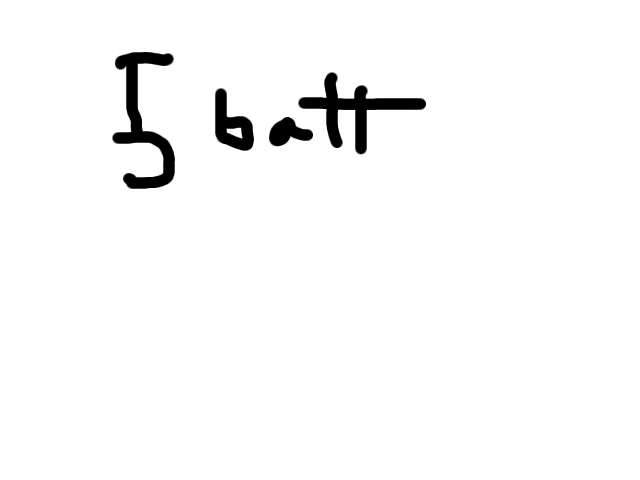
\includegraphics[width=0.4\textwidth]{fig/fivebatteries}
\caption{Eating \(5\) batteries}
\end{figure}

\begin{table}[h]
\label{tab:ssb}
\caption{Captain Falcon}
\centering
\begin{tabular}{r | l}
Falcons & Not Falcons\\
\hline
FALCON & KICK\\
FALCON & KICK\\
FALCON & PUNCH!!
\end{tabular}
\end{table}


\end{document}
\end{verbatim}
\normalsize

This is how appendices are included. In fact, they are written just like
regular chapters, and the \textbackslash appendix flag signals that following
chapters should be given letters (A, B, C...) instead of numbers (1, 2, 3...).

\chapter{Gotchas and Caveats}

\section{Introduction}

\texttt{uafthesis} is not perfect. It still has issues that you need to keep
in mind.

\section{List of Appendices Chicanery}

In an ideal world, \texttt{uafthesis} would write your appendices to the
list of appendices instead of the table of contents. This is currently a bug,
and will be fixed in the future.

The workaround is this:

\begin{enumerate}
\item After generating a pretty-much-done thesis, open up the .toc file. In
this case, the file is called ``example.toc.'' Also open up a corresponding
.loa file (``example.loa'').
\item Cut the lines that refer to appendices out of the .toc file and paste
them into the .loa file. Save both. Make sure the first line in the .loa
that adds "Page" above the pages column stays put.
\item \emph{Make backups of both files.} This is because \LaTeX will overwrite
the .toc file in the next step.
\item Compile (\texttt{pdflatex example}) \emph{exactly once.}
\end{enumerate}

\section{List of Other Materials}

A similar process applies to the List of Other Materials as well:

\begin{quotation}
{ \it ``If you add a pocket or anything else to your thesis (like a CD-ROM)
then you have to have one more List in the Table of Contents.  Follow
the exact same procedure as in step 14, but now you must add the
command:

\textbackslash listofothermaterials

Notice that this goes before the \textbackslash listofappendices.  The file that you
must edit is the thesis12.lom file.  You have to create this by hand.
It is simple.  Here is the example:

\textbackslash renewcommand\textbackslash @pnumwidth\{3.55em\}
\textbackslash contentsline \{section\}{\textbackslash numberline \{A\}CD-ROM of Thesis, Defense and Sandpile Code\}\{Pocket\}
\textbackslash renewcommand\textbackslash @pnumwidth\{1.55em\}

Again, once you save this and run latex once, it will be erased.  A
good habit is to make thesis12.lom.bak and thesis12.loa.bak so they
will always be there.  Then copy them to thesis12.lom and thesis12.loa
and run latex your final time.

I did the \textbackslash @pnumwidth stuff above because the word `Pocket' is wider
than is allowed for a page number.  So I changed it just for this one
line and then changed it back to what it was (as found in the
uafthesis2004.cls file).''\\
\hspace*{1in}---Ryan Woodard
\end{quotation}

I suspect that there's a better way to do this, but I haven't gotten that far
yet.

\section{Bibliography Listings}

If you use \texttt{chapterbib}, also use \texttt{tocbibind} to make sure that
your bibliographies show up in the Table of Contents.

\end{verbatim}
\normalsize

After inputting a few more pages, the chapters (separate documents) are all
included.

\small
\begin{verbatim}
\nocite{wikibook}
\bibliographystyle{agufull08}
\bibliography{thesis}
\end{verbatim}
\normalsize

This generates the bibliography. Note that the bibliography style is set to
\texttt{agufull08}. Generally, the graduate school isn't picky about 
bibliography style, as long as it's consistent. For geophysics papers (very
common at UAF), the AGU style is a great choice. It is included here, but may
also be found at AGU's web site.

\small
\begin{verbatim}
\appendix
\chapter{Extraneous Images and Tables}

\begin{figure}[h]
\label{fig:onebattery}
\centering

\includegraphics[width=0.4\textwidth]{fig/onebattery}
\caption{Eating \(1\) battery}
\end{figure}

\begin{figure}[h]
\label{fig:fivebatteries}
\centering
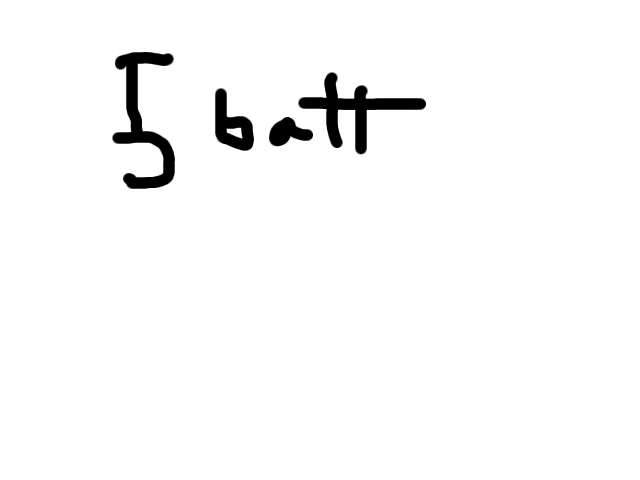
\includegraphics[width=0.4\textwidth]{fig/fivebatteries}
\caption{Eating \(5\) batteries}
\end{figure}

\begin{table}[h]
\label{tab:ssb}
\caption{Captain Falcon}
\centering
\begin{tabular}{r | l}
Falcons & Not Falcons\\
\hline
FALCON & KICK\\
FALCON & KICK\\
FALCON & PUNCH!!
\end{tabular}
\end{table}


\end{document}
\end{verbatim}
\normalsize

This is how appendices are included. In fact, they are written just like
regular chapters, and the \textbackslash appendix flag signals that following
chapters should be given letters (A, B, C...) instead of numbers (1, 2, 3...).


\nocite{wikibook}
\bibliographystyle{agufull08}
\bibliography{example}

\appendix
\chapter{Extraneous Images and Tables}

\begin{figure}[h]
\label{fig:onebattery}
\centering

\includegraphics[width=0.4\textwidth]{fig/onebattery}
\caption{Eating \(1\) battery}
\end{figure}

\begin{figure}[h]
\label{fig:fivebatteries}
\centering
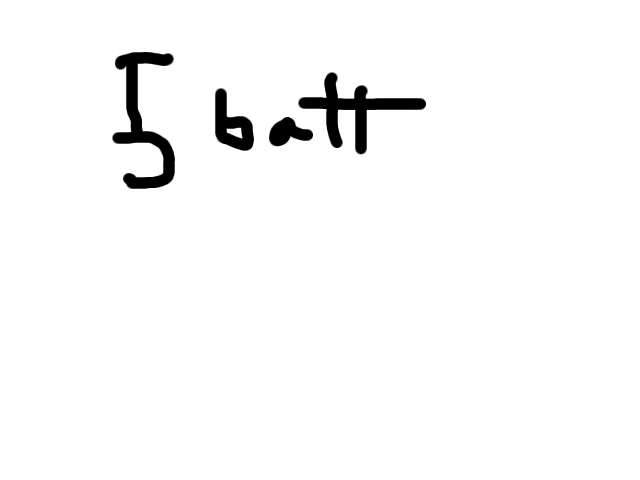
\includegraphics[width=0.4\textwidth]{fig/fivebatteries}
\caption{Eating \(5\) batteries}
\end{figure}

\begin{table}[h]
\label{tab:ssb}
\caption{Captain Falcon}
\centering
\begin{tabular}{r | l}
Falcons & Not Falcons\\
\hline
FALCON & KICK\\
FALCON & KICK\\
FALCON & PUNCH!!
\end{tabular}
\end{table}


\end{document}
